%%%%%%%%%%%%%%%%%%%%%%%%%%%%%%%%%%%%%%%%%
% a0poster Portrait Poster
% LaTeX Template
% Version 1.0 (22/06/13)
%
% The a0poster class was created by:
% Gerlinde Kettl and Matthias Weiser (tex@kettl.de)
% 
% This template has been downloaded from:
% http://www.LaTeXTemplates.com
%
% License:
% CC BY-NC-SA 3.0 (http://creativecommons.org/licenses/by-nc-sa/3.0/)
%
%%%%%%%%%%%%%%%%%%%%%%%%%%%%%%%%%%%%%%%%%

%----------------------------------------------------------------------------------------
%	PACKAGES AND OTHER DOCUMENT CONFIGURATIONS
%----------------------------------------------------------------------------------------

\documentclass[a0,portrait]{a0poster}

\usepackage{multicol} % This is so we can have multiple columns of text side-by-side
\columnsep=100pt % This is the amount of white space between the columns in the poster
\columnseprule=3pt % This is the thickness of the black line between the columns in the poster

\usepackage[svgnames]{xcolor} % Specify colors by their 'svgnames', for a full list of all colors available see here: http://www.latextemplates.com/svgnames-colors
\usepackage{CJKutf8, CJK}
\usepackage{times} % Use the times font
%\usepackage{palatino} % Uncomment to use the Palatino font
\usepackage{makecell}                 % 三线表-竖线
\usepackage{booktabs}                 % 三线表-短细横线
\usepackage{graphicx}				  % 表格单元格逆时针
\usepackage{multirow}				  % 合并单元格
\usepackage{array}
\usepackage{amssymb}				  % 勾
\usepackage{longtable}                % 导入 longtable 宏包,表格自动换行
\usepackage{amsmath}
\usepackage{graphicx} % Required for including images
\graphicspath{{figures/}} % Location of the graphics files
\usepackage{booktabs} % Top and bottom rules for table
\usepackage[font=small,labelfont=bf]{caption} % Required for specifying captions to tables and figures
\usepackage{amsfonts, amsmath, amsthm, amssymb} % For math fonts, symbols and environments
\usepackage{wrapfig} % Allows wrapping text around tables and figures
\usepackage{graphicx}
\usepackage{caption}
\usepackage{subcaption}
\usepackage[final]{hyperref} % adds hyper links inside the generated pdf file
\hypersetup{
	colorlinks=true,       % false: boxed links; true: colored links
	linkcolor=blue,        % color of internal links
	citecolor=blue,        % color of links to bibliography
	filecolor=magenta,     % color of file links
	urlcolor=blue         
}


\begin{document}

%----------------------------------------------------------------------------------------
%	POSTER HEADER 
%----------------------------------------------------------------------------------------

% The header is divided into two boxes:
% The first is 75% wide and houses the title, subtitle, names, university/organization and contact information
% The second is 25% wide and houses a logo for your university/organization or a photo of you
% The widths of these boxes can be easily edited to accommodate your content as you see fit

\begin{minipage}[b]{0.75\linewidth}
\Huge \color{NavyBlue} \textbf{Facial expression recognition based on opencv and keras} \color{Black}\\ % Title
\LARGE \textit{}\\[2cm] % Subtitle
\LARGE \textbf{Li Xinyue}\\[0.5cm] % Author(s)
\LARGE LanZhou University, UAIS CAI-minions Resort\\ [0.4cm] % University/organization
\large Lanzhou University Annual meeting paper 
\\
\end{minipage}
%
\hspace{-5.5cm}\begin{minipage}[b]{0.3\linewidth}
% \includegraphics[scale=0.5]{ciencias.png}\qquad

\includegraphics[scale=2.5]{lzu.png}
\end{minipage}

\vspace{1cm} % A bit of extra whitespace between the header and poster content

%----------------------------------------------------------------------------------------

\begin{multicols}{2} % This is how many columns your poster will be broken into, a portrait poster is generally split into 2 columns

%----------------------------------------------------------------------------------------
%	ABSTRACT
%----------------------------------------------------------------------------------------


\color{DarkRed}

\begin{abstract}
	With the rapid development of deep learning and machine learning, facial expression recognition is the most direct understanding way of human emotion, ushered in a new way of processing. From traditional recognition methods to recognition methods based on deep learning, facial expression recognition has developed by leaps and bounds. Automatic analysis of facial expressions is very important for computers to understand human emotional state. it is an important way to understand human emotions based on computer vision. it has important influence and is used in many fields, such as human-computer interaction data-driven animation and so on.
\end{abstract}

%----------------------------------------------------------------------------------------
%	INTRODUCTION
%----------------------------------------------------------------------------------------

\color{Black}
\section*{Introduction}

\quad This paper uses Keras and Opencv for facial expression recognition by constructing a convolution neural network model. The choice of Keras is due to its ease of use and compatibility with TensorFlow. The network structure is crucial for accuracy, so the paper experiments with different models, including traditional neural networks, Xception, and residual networks. To prevent overfitting, model parameters are adjusted through repeated experiments.

%----------------------------------------------------------------------------------------
%	CHALLENGE
%----------------------------------------------------------------------------------------


\section*{Challenge}

\quad Since the expression recognition methods based on deep learning are affected by many hyperparameters, the comparability of the current facial expression recognition methods is not strong, and it is necessary to evaluate different expression recognition methods on different simple baseline methods.

%----------------------------------------------------------------------------------------
%	MATERIALS AND METHODS
%----------------------------------------------------------------------------------------

\section*{Methods}

\subsection*{Preprocess Data}

\quad We choose the fer2013 data set, which has a total of 35887 images. The dataset(Fig.\ref{fig: fer2013_dataset}) is divided into three categories, each of which is as follows: 28709 training sets (Training), 3859 verification sets (Val) and 3859 test sets (Test).

\begin{center}\vspace{1cm}
	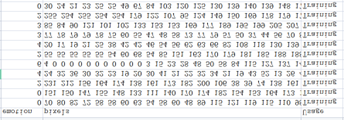
\includegraphics[width=0.5\linewidth]{fer2013_dataset}
	\captionof{figure}{
		\label{fig: fer2013_dataset}
		fer2013 dataset.}
\end{center}\vspace{1cm}

\subsection*{Data Enhancement}

\quad Data enhancement can be used to improve model performance by adding an appropriate amount of noise to the original data to improve model expressiveness and avoid overfitting. ImageDataGenerator can be used to perform data enhancement by generating an iterative object that specifies the desired enhancement operations\cite{b1}, such as image decentralization, random flipping, and offsetting. After processing the images, they can be accessed through Next and saved in the Output file. The four-dimensional array received by Flow specifies the number, length, width, and grayscale of the image.

\begin{center}\vspace{1cm}
	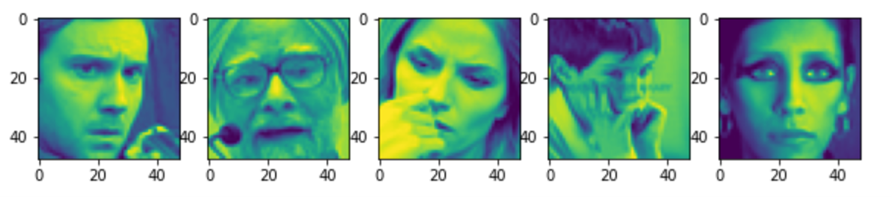
\includegraphics[width=0.8\linewidth]{original_data}
	\captionof{figure}{
		\label{fig: original_data}
		Visualization of original data.}
\end{center}\vspace{1cm}


By comparing the enhanced image (Fig.\ref{fig: original_data}) with the original image (Fig.\ref{fig: data_enhanced_visualization}), the enhanced image works better.


\begin{center}\vspace{1cm}
	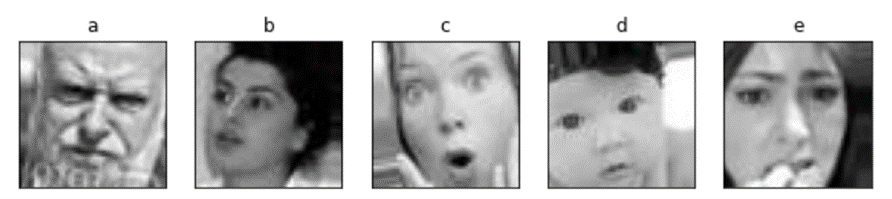
\includegraphics[width=0.8\linewidth]{data_enhanced_visualization}
	\captionof{figure}{
		\label{fig: data_enhanced_visualization}
		The data enhanced visualization.}
\end{center}\vspace{1cm}


\subsection*{Scale Normalization}

\quad To handle input images of varying sizes and ensure that key facial features are retained while irrelevant information is discarded, the images are cropped to a uniform size. However, the size of the crop should be appropriate - if it is too large, extraneous information will be included, making feature extraction more difficult and reducing model accuracy. Conversely, if the crop is too small, important information may be lost. Therefore, the human eye is typically used as a reference point for cropping and aligning the images.

\begin{center}\vspace{1cm}
	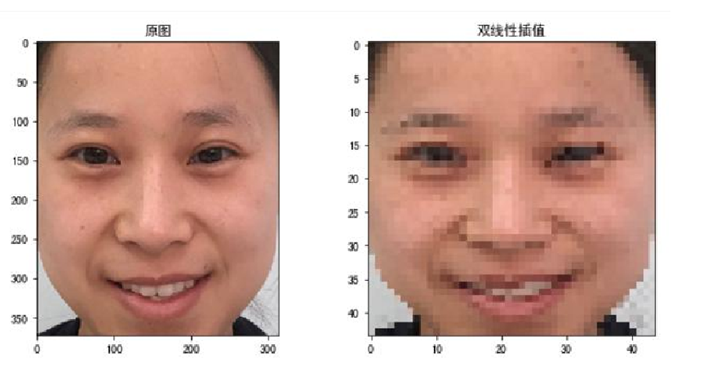
\includegraphics[width=0.4\linewidth]{compared}
	\captionof{figure}{
		\label{fig: compared}
		Compared the double-valued interpolation method’s result with the original figure.}
\end{center}\vspace{1cm}

%----------------------------------------------------------------------------------------
%	MODEL
%----------------------------------------------------------------------------------------
\section*{Model}


Three models were compared in this experiment: Xception, traditional neural network, and residual network model\cite{b2}. The Xception model takes single-channel grayscale images with a shape of [48 × 48 × 1], and the traditional neural network and residual network models use multiple layers for feature extraction. To reduce memory cost and training time, the training data is randomly divided into batches. During training, each batch is fed into the model to calculate the predicted value, and the optimizer updates the model parameters to minimize the loss function based on the derivative of the loss function compared with the actual value. The training process saves optimal weight data using Keras callback mechanisms and monitors loss and accuracy to prevent overfitting or stagnation. A callback function is set to dynamically adjust the learning rate when the standard evaluation does not improve, and the training is stopped if the loss on the verification set remains the same after multiple adjustments.

%----------------------------------------------------------------------------------------
%	RESULTS 
%----------------------------------------------------------------------------------------

\section*{Results}

\quad This chapter conducts an experiment using the fer2013 dataset with image size of [48 × 48]. The Xception, traditional, and residual network models are used for comparison, with a batch size of 32 and a total of 35887 images. Due to unstable computing resources, hierarchical training (50 or 100) is used, and GPU of the Googlecolaboratory is used for cloud training. The weight data is always in memory and video memory, and the training results can be reused in time. See Table\ref{tab: Model training comparison table} for the comparison results.

\begin{center}\vspace{1cm}
		\captionof{table}{
		\label{tab: Model training comparison table}
		Model training comparison table
	}
	\begin{tabular}{ccccccc}
		
		\toprule %添加表格头部粗线
		
		% \multirow{2}*{\textbf{Learning}} & \multirow{2}*{\textbf{Mathod}} & \multicolumn{4}{c|}{\textbf{LOL-test}} & \multicolumn{4}{c}{\textbf{MIT-Adobe FiveK-test}} \\
		
		
		\textbf{Model} & \textbf{Image size} & \textbf{Batch size} & \textbf{epochs} & \textbf{Train\_acc}  & \textbf{optimizer} &  \textbf{Val\_acc}\\
		
		\hline
		
		Xception & 48×48 & 32 & 200 & 0.72 & adam & 0.63 \\
		Tradition& 48×48 & 32 & 200 & 0.68 & adam & 0.61 \\
		Resnet   & 48×48 & 32 & 200	& 0.81 & adam & 0.66 \\
		
		\bottomrule
		
	\end{tabular}
\end{center}\vspace{1cm}

The traditional model achieved a training set accuracy of 0.68 and a verification set accuracy of 0.61 with over 300,000 parameters(Fig.\ref{fig: parameters}). On the other hand, the Xception model achieved a training set accuracy close to 0.72, a verification set accuracy of about 0.63, and had only 50,000 parameters, leading to a better performance compared to the traditional model.

\begin{center}\vspace{1cm}
	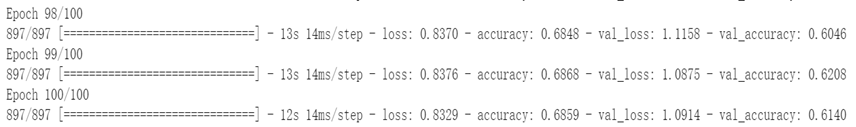
\includegraphics[width=0.8\linewidth]{training_results}
	\captionof{figure}{
		\label{fig: training_results}
		The display of traditional model training results }
\end{center}\vspace{1cm}

\begin{center}\vspace{1cm}
	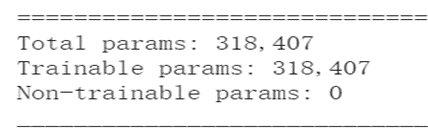
\includegraphics[width=0.5\linewidth]{parameters}
	\captionof{figure}{
		\label{fig: parameters}
		The parameters used in traditional models.}
\end{center}\vspace{1cm}

By selecting an image and selecting an image in the file for facial expression recognition, then you can see that the recognition result is anger as shown in Fig.\ref{fig: expression_recognition_results} below. The probability of anger recognition in the column on the right is 95\%, and the rest of the disgust is slightly higher by 4\%

\begin{center}\vspace{1cm}
	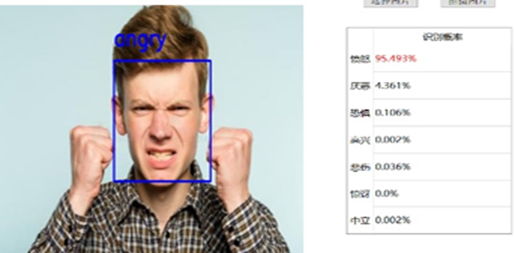
\includegraphics[width=0.5\linewidth]{expression_recognition_results}
	\captionof{figure}{
		\label{fig: expression_recognition_results}
		The display of facial expression recognition results.}
\end{center}\vspace{1cm}


%----------------------------------------------------------------------------------------
%	CONCLUSIONS
%----------------------------------------------------------------------------------------

\section*{Summary}

%\begin{itemize}
%\item we propose a method to cope with the anomaly detection challenges that brought by the natural characteristics of multivariate CDN KPIs of diverse websites.
%\end{itemize}

\quad This paper presents a comprehensive empirical study of facial expressions, which involves addressing various challenges such as variations in image size and quality, low-resolution images, and model selection and parameter optimization to improve recognition accuracy. These issues are critical for achieving accurate facial expression recognition, as different models can yield varying results on the same dataset.


%----------------------------------------------------------------------------------------
%	REFERENCES
%----------------------------------------------------------------------------------------

\begin{thebibliography}{00}
	\bibitem{b1}\label{cite:b1}
		Hong Guo,Jiayou Chen. Dynamic Facial Expression Recognition Based on ResNet and LSTM[C]//Proceedings of 2019 2nd International Conference on Communication,network and Artificial Intelligence(cnai 2019): Iop Publishing, 2019: 990-996.
	
	\bibitem{b2}\label{cite:b2}	
		Zhe Sun,Hehao Zhang,Suwei Ma, et al. Combining filtered dictionary representation based deep subspace filter learning with a discriminative classification criterion for facial expression recognition[J]. Artificial Intelligence Review, 2022(prepublish).
	
\end{thebibliography}


\end{multicols}
\end{document}